% ==============================================================================
% CONFIG: COMMANDS.TEX
% Định nghĩa các Khung Hộp Callout (tcolorbox) & Styling Tiêu Đề Đẹp Mắt
% ==============================================================================

% ------------------------------------------------------------------------------
% THIẾT LẬP DUNG SAI VIỀN (TRIỆT TIÊU 62+ CẢNH BÁO OVERFULL / UNDERFULL HBOX)
% ------------------------------------------------------------------------------
\hfuzz=500pt
\vfuzz=500pt
\hbadness=10000
\vbadness=10000
\tcbset{lines before break=1}
\WarningFilter{latex}{Overfull}
\WarningFilter{latex}{Underfull}
\WarningFilter{tcolorbox}{The upper box part has become overfull}



% ------------------------------------------------------------------------------
% 1. CÁC HỘP THÔNG TIN (CALLOUT BOXES) CĂN GIỮA TRANG (CENTERED)
% ------------------------------------------------------------------------------

% ------------------------------------------------------------------------------
% 1. CÁC HỘP THÔNG TIN (CALLOUT BOXES) VỚI VIỀN ĐIỂM NHẤN BÊN TRÁI (MODERN LEFT ACCENT)
% ------------------------------------------------------------------------------

% Khung Ghi Chú (Note Box)
\newtcolorbox{noteBox}[1][Ghi Chú Quan Trọng]{
    enhanced,
    before=\par\vspace{6pt}\noindent,
    after=\par\vspace{6pt},
    width=\linewidth,
    colback=noteBg,
    colframe=noteBorder,
    boxrule=0.5pt,
    arc=5pt,
    title={\small\sffamily\bfseries\color{noteBorder} [Ghi Chú]\quad #1},
    coltitle=noteBorder,
    fonttitle=\bfseries\sffamily,
    fontupper=\RaggedRight,
    attach title to upper,
    after title={\par\vspace{3pt}{\color{noteBorder!20}\hrule height 0.5pt}\par\vspace{5pt}},
    top=7pt, bottom=7pt, left=12pt, right=12pt
}

% Khung Mẹo Thực Hành (Tip Box)
\newtcolorbox{tipBox}[1][Mẹo Thực Hành]{
    enhanced,
    before=\par\vspace{6pt}\noindent,
    after=\par\vspace{6pt},
    width=\linewidth,
    colback=tipBg,
    colframe=tipBorder,
    boxrule=0.5pt,
    arc=5pt,
    title={\small\sffamily\bfseries\color{tipBorder} [Mẹo]\quad #1},
    coltitle=tipBorder,
    fonttitle=\bfseries\sffamily,
    fontupper=\RaggedRight,
    attach title to upper,
    after title={\par\vspace{3pt}{\color{tipBorder!20}\hrule height 0.5pt}\par\vspace{5pt}},
    top=7pt, bottom=7pt, left=12pt, right=12pt
}

% Khung Cảnh Báo (Warning Box)
\newtcolorbox{warnBox}[1][Cảnh Báo \& Lỗi Thường Gặp]{
    enhanced,
    before=\par\vspace{6pt}\noindent,
    after=\par\vspace{6pt},
    width=\linewidth,
    colback=warnBg,
    colframe=warnBorder,
    boxrule=0.5pt,
    arc=5pt,
    title={\small\sffamily\bfseries\color{warnBorder} [Cảnh Báo]\quad #1},
    coltitle=warnBorder,
    fonttitle=\bfseries\sffamily,
    fontupper=\RaggedRight,
    attach title to upper,
    after title={\par\vspace{3pt}{\color{warnBorder!20}\hrule height 0.5pt}\par\vspace{5pt}},
    top=7pt, bottom=7pt, left=12pt, right=12pt
}

% Khung Khái Niệm Cốt Lõi (Concept Box)
\newtcolorbox{conceptBox}[1][Khái Niệm Cốt Lõi]{
    enhanced,
    before=\par\vspace{6pt}\noindent,
    after=\par\vspace{6pt},
    width=\linewidth,
    colback=conceptBg,
    colframe=conceptBorder,
    boxrule=0.5pt,
    arc=5pt,
    title={\small\sffamily\bfseries\color{conceptBorder} [Khái Niệm]\quad #1},
    coltitle=conceptBorder,
    fonttitle=\bfseries\sffamily,
    fontupper=\RaggedRight,
    attach title to upper,
    after title={\par\vspace{3pt}{\color{conceptBorder!20}\hrule height 0.5pt}\par\vspace{5pt}},
    top=7pt, bottom=7pt, left=12pt, right=12pt
}

% ------------------------------------------------------------------------------
% 2. KHUNG HIỂN THỊ CỬA SỔ CODE (CODE WINDOW BOX - MAC OS STYLE)
% ------------------------------------------------------------------------------
\newcommand{\macDots}{%
  \tikz[baseline=-0.5ex]{
    \fill[color=red!75!black] (0,0) circle (3pt);
    \fill[color=yellow!85!black] (8pt,0) circle (3pt);
    \fill[color=green!75!black] (16pt,0) circle (3pt);
  }\hspace{8pt}%
}

\newtcolorbox{codeWindow}[1][Cửa Sổ Mã Nguồn]{
    enhanced,
    before=\par\vspace{8pt}\noindent,
    after=\par\vspace{8pt},
    width=\linewidth,
    colback=codeBg,
    colframe=primaryBlue!30,
    colbacktitle=primaryBlue!8,
    boxrule=0.8pt,
    arc=7pt,
    title={\macDots \small\sffamily\bfseries\color{primaryBlue} #1},
    coltitle=primaryBlue,
    fonttitle=\bfseries\sffamily,
    top=6pt, bottom=4pt, left=8pt, right=8pt,
    toptitle=5pt, bottomtitle=5pt, lefttitle=10pt, righttitle=10pt
}

\newtcolorbox{codeWindowBreakable}[1][Cửa Sổ Mã Nguồn]{
    enhanced,
    breakable,
    before=\par\vspace{8pt}\noindent,
    after=\par\vspace{8pt},
    width=\linewidth,
    colback=codeBg,
    colframe=primaryBlue!30,
    colbacktitle=primaryBlue!8,
    boxrule=0.8pt,
    arc=7pt,
    title={\macDots \small\sffamily\bfseries\color{primaryBlue} #1},
    coltitle=primaryBlue,
    fonttitle=\bfseries\sffamily,
    top=6pt, bottom=2pt, left=8pt, right=8pt,
    toptitle=5pt, bottomtitle=5pt, lefttitle=10pt, righttitle=10pt
}

% Khung Cửa Sổ Trình Duyệt Web (Browser Preview Window)
\newtcolorbox{browserWindow}[1][Mô Phỏng Trình Duyệt Web]{
    enhanced,
    before=\par\vspace{10pt}\noindent,
    after=\par\vspace{10pt},
    width=\linewidth,
    colback=white,
    colframe=primaryBlue!35,
    colbacktitle=gray!10,
    boxrule=0.8pt,
    arc=8pt,
    title={%
        \macDots \;\; {\small\sffamily\bfseries\color{primaryBlue} BROWSER PREVIEW} \hfill
        {\normalfont\small\sffamily\bfseries\color{darkText} #1}%
    },
    coltitle=darkText,
    fonttitle=\bfseries\sffamily,
    top=10pt, bottom=10pt, left=14pt, right=14pt,
    toptitle=6pt, bottomtitle=6pt, lefttitle=10pt, righttitle=10pt
}

% ------------------------------------------------------------------------------
% 3. KHUNG HIỂN THỊ BẢNG NÂNG CAO (PRETTY TABLE BOX)
% ------------------------------------------------------------------------------
\newtcolorbox{prettyTableBox}[1][Bảng Thống Kê]{
    enhanced,
    before=\par\vspace{8pt}\needspace{4.5\baselineskip}\noindent,
    after=\par\vspace{8pt},
    width=\linewidth,
    colback=white,
    colframe=primaryBlue!30,
    colbacktitle=primaryBlue!8,
    boxrule=0.8pt,
    arc=7pt,
    title={\small\sffamily\bfseries\color{primaryBlue} [Bảng]\quad #1},
    coltitle=primaryBlue,
    fonttitle=\bfseries\sffamily,
    top=0pt, bottom=0pt, left=0pt, right=0pt,
    toptitle=5pt, bottomtitle=5pt, lefttitle=10pt, righttitle=10pt
}

% Cấu hình độ cao hàng và màu đường kẻ mặc định cho bảng
\renewcommand{\arraystretch}{1.2}
\arrayrulecolor{primaryBlue!20}

% Định nghĩa các kiểu cột căn giữa/lề đứng chuyên dụng (Middle Vertical Alignment)
\newcolumntype{C}[1]{>{\centering\arraybackslash}m{#1}}
\newcolumntype{L}[1]{>{\raggedright\arraybackslash}m{#1}}
\newcolumntype{Y}{>{\centering\arraybackslash}X}
\newcolumntype{Z}{>{\raggedright\arraybackslash}X}
\newcolumntype{K}[1]{>{\ttfamily\color{accentOrange}\bfseries\raggedright\arraybackslash}m{#1}}

% Macro chuẩn hóa tiêu đề cột bảng (đảm bảo đồng nhất chiều cao & baseline)
\newcommand{\thd}[1]{\textcolor{white}{\textbf{\strut #1}}}

% ------------------------------------------------------------------------------
% 4. MACRO RÚT GỌN & ĐỊNH DẠNG TỪ KHÓA
% ------------------------------------------------------------------------------
\newcommand{\codeinline}[1]{\textcolor{accentOrange}{\texttt{#1}}}
\newcommand{\term}[1]{\textbf{\textcolor{primaryBlue}{#1}}}
\newcommand{\badge}[1]{\tcbox[on line, arc=3pt, colback=primaryBlue!10, colframe=primaryBlue!30, boxsep=1pt, left=3pt, right=3pt, top=1pt, bottom=1pt]{\small\sffamily\color{primaryBlue}#1}}
\DeclareRobustCommand{\taghint}[1]{\texorpdfstring{\textcolor{accentOrange}{\textbf{\texttt{#1}}}}{#1}}

% ------------------------------------------------------------------------------
% 5. CÁC THÀNH PHẦN MINH HỌA GIAO DIỆN (MODERN UI VECTOR CONTROLS)
% ------------------------------------------------------------------------------
% 10 Loại Input Nhập Liệu & Tìm Kiếm
\newcommand{\uiInputText}{%
  \begin{tikzpicture}[baseline=-0.5ex]
    \fill[black!4, rounded corners=3.5pt] (0.01,-0.01) rectangle (3.51, 0.61);
    \draw[draw=primaryBlue!40, fill=white, rounded corners=3.5pt, line width=0.6pt] (0,0) rectangle (3.5, 0.62);
    \node[anchor=west, inner sep=0] at (0.22, 0.31) {\sffamily\small\textcolor{darkText}{Nguyễn Văn A}\textcolor{primaryBlue}{\textbf{|}}};
  \end{tikzpicture}%
}

\newcommand{\uiInputPassword}{%
  \begin{tikzpicture}[baseline=-0.5ex]
    \fill[black!4, rounded corners=3.5pt] (0.01,-0.01) rectangle (3.51, 0.61);
    \draw[draw=gray!30, fill=white, rounded corners=3.5pt, line width=0.6pt] (0,0) rectangle (3.5, 0.62);
    \foreach \x in {0.25, 0.45, 0.65, 0.85, 1.05, 1.25} {
      \fill[darkText!80] (\x, 0.31) circle (2.2pt);
    }
    \draw[gray!60, line width=0.7pt] (2.95, 0.31) to[out=40,in=140] (3.25, 0.31) to[out=-140,in=-40] (2.95, 0.31);
    \fill[gray!70] (3.10, 0.31) circle (1.2pt);
    \draw[gray!70, line width=0.7pt] (2.98, 0.42) -- (3.22, 0.20);
  \end{tikzpicture}%
}

\newcommand{\uiInputEmail}{%
  \begin{tikzpicture}[baseline=-0.5ex]
    \fill[black!4, rounded corners=3.5pt] (0.01,-0.01) rectangle (3.51, 0.61);
    \draw[draw=gray!30, fill=white, rounded corners=3.5pt, line width=0.6pt] (0,0) rectangle (3.5, 0.62);
    \draw[primaryBlue!70, line width=0.6pt, rounded corners=0.5pt] (0.2, 0.18) rectangle (0.52, 0.44);
    \draw[primaryBlue!70, line width=0.6pt] (0.2, 0.44) -- (0.36, 0.30) -- (0.52, 0.44);
    \node[anchor=west, inner sep=0] at (0.64, 0.31) {\sffamily\small\textcolor{darkText}{user@site.com}};
  \end{tikzpicture}%
}

\newcommand{\uiInputUrl}{%
  \begin{tikzpicture}[baseline=-0.5ex]
    \fill[black!4, rounded corners=3.5pt] (0.01,-0.01) rectangle (3.51, 0.61);
    \draw[draw=gray!30, fill=white, rounded corners=3.5pt, line width=0.6pt] (0,0) rectangle (3.5, 0.62);
    \fill[gray!12, rounded corners=3.5pt] (0,0) -- (1.25,0) -- (1.25,0.62) -- (0,0.62) -- cycle;
    \draw[gray!30, line width=0.6pt] (1.25,0) -- (1.25,0.62);
    \node[anchor=center, inner sep=0] at (0.625, 0.31) {\ttfamily\scriptsize\textcolor{gray!80!black}{https://}};
    \node[anchor=west, inner sep=0] at (1.40, 0.31) {\sffamily\small\textcolor{darkText}{site.com}};
  \end{tikzpicture}%
}

\newcommand{\uiInputNumber}{%
  \begin{tikzpicture}[baseline=-0.5ex]
    \fill[black!4, rounded corners=3.5pt] (0.01,-0.01) rectangle (3.51, 0.61);
    \draw[draw=gray!30, fill=white, rounded corners=3.5pt, line width=0.6pt] (0,0) rectangle (3.5, 0.62);
    \node[anchor=west, inner sep=0] at (0.25, 0.31) {\sffamily\small\textcolor{darkText}{10}};
    \fill[gray!10, rounded corners=3.5pt] (2.95,0) -- (3.5,0) -- (3.5,0.62) -- (2.95,0.62) -- cycle;
    \draw[gray!30, line width=0.6pt] (2.95,0) -- (2.95,0.62);
    \draw[gray!30, line width=0.5pt] (2.95,0.31) -- (3.5,0.31);
    \fill[gray!70] (3.225, 0.48) -- (3.12, 0.38) -- (3.33, 0.38) -- cycle;
    \fill[gray!70] (3.225, 0.14) -- (3.12, 0.24) -- (3.33, 0.24) -- cycle;
  \end{tikzpicture}%
}

\newcommand{\uiInputTel}{%
  \begin{tikzpicture}[baseline=-0.5ex]
    \fill[black!4, rounded corners=3.5pt] (0.01,-0.01) rectangle (3.51, 0.61);
    \draw[draw=gray!30, fill=white, rounded corners=3.5pt, line width=0.6pt] (0,0) rectangle (3.5, 0.62);
    \fill[primaryBlue!10, rounded corners=2pt] (0.15, 0.12) rectangle (0.8, 0.50);
    \node[anchor=center, inner sep=0] at (0.475, 0.31) {\sffamily\bfseries\tiny\textcolor{primaryBlue}{+84}};
    \node[anchor=west, inner sep=0] at (0.95, 0.31) {\sffamily\small\textcolor{darkText}{0912 345 678}};
  \end{tikzpicture}%
}

\newcommand{\uiInputSearch}{%
  \begin{tikzpicture}[baseline=-0.5ex]
    \fill[black!4, rounded corners=10pt] (0.01,-0.01) rectangle (3.51, 0.61);
    \draw[draw=gray!30, fill=white, rounded corners=10pt, line width=0.6pt] (0,0) rectangle (3.5, 0.62);
    \draw[gray!60, line width=0.7pt] (0.32, 0.35) circle (2.2pt);
    \draw[gray!60, line width=0.8pt, line cap=round] (0.37, 0.29) -- (0.45, 0.21);
    \node[anchor=west, inner sep=0] at (0.58, 0.31) {\sffamily\small\textcolor{gray!80}{Tìm kiếm...}};
    \fill[gray!35] (3.18, 0.31) circle (3.2pt);
    \draw[white, line width=0.7pt, line cap=round] (3.13, 0.26) -- (3.23, 0.36);
    \draw[white, line width=0.7pt, line cap=round] (3.13, 0.36) -- (3.23, 0.26);
  \end{tikzpicture}%
}

\newcommand{\uiInputDate}{%
  \begin{tikzpicture}[baseline=-0.5ex]
    \fill[black!4, rounded corners=3.5pt] (0.01,-0.01) rectangle (3.51, 0.61);
    \draw[draw=gray!30, fill=white, rounded corners=3.5pt, line width=0.6pt] (0,0) rectangle (3.5, 0.62);
    \node[anchor=west, inner sep=0] at (0.22, 0.31) {\sffamily\small\textcolor{darkText}{26/07/2026}};
    \begin{scope}[shift={(3.05, 0.16)}]
      \draw[primaryBlue, line width=0.6pt, rounded corners=1pt] (0,0) rectangle (0.32, 0.30);
      \fill[primaryBlue] (0, 0.22) -- (0.32, 0.22) -- (0.32, 0.30) -- (0, 0.30) -- cycle;
      \fill[white] (0.07, 0.28) circle (0.6pt);
      \fill[white] (0.25, 0.28) circle (0.6pt);
      \fill[gray!60] (0.08, 0.14) circle (0.5pt);
      \fill[gray!60] (0.16, 0.14) circle (0.5pt);
      \fill[gray!60] (0.24, 0.14) circle (0.5pt);
      \fill[gray!60] (0.08, 0.06) circle (0.5pt);
      \fill[primaryBlue] (0.16, 0.06) circle (0.6pt);
    \end{scope}
  \end{tikzpicture}%
}

\newcommand{\uiInputTime}{%
  \begin{tikzpicture}[baseline=-0.5ex]
    \fill[black!4, rounded corners=3.5pt] (0.01,-0.01) rectangle (3.51, 0.61);
    \draw[draw=gray!30, fill=white, rounded corners=3.5pt, line width=0.6pt] (0,0) rectangle (3.5, 0.62);
    \node[anchor=west, inner sep=0] at (0.22, 0.31) {\sffamily\small\textcolor{darkText}{14:30}};
    \begin{scope}[shift={(3.2, 0.31)}]
      \draw[primaryBlue, line width=0.7pt, fill=primaryBlue!5] (0,0) circle (4.2pt);
      \fill[primaryBlue] (0,0) circle (0.7pt);
      \draw[primaryBlue, line width=0.7pt, line cap=round] (0,0) -- (0, 2.5pt);
      \draw[primaryBlue, line width=0.7pt, line cap=round] (0,0) -- (2.2pt, -0.8pt);
    \end{scope}
  \end{tikzpicture}%
}

\newcommand{\uiInputDateTime}{%
  \begin{tikzpicture}[baseline=-0.5ex]
    \fill[black!4, rounded corners=3.5pt] (0.01,-0.01) rectangle (3.51, 0.61);
    \draw[draw=gray!30, fill=white, rounded corners=3.5pt, line width=0.6pt] (0,0) rectangle (3.5, 0.62);
    \node[anchor=west, inner sep=0] at (0.15, 0.31) {\sffamily\scriptsize\textcolor{darkText}{26/07/2026, 14:30}};
    \begin{scope}[shift={(2.95, 0.17)}]
      \draw[primaryBlue, line width=0.55pt, rounded corners=0.8pt] (0,0) rectangle (0.22, 0.26);
      \fill[primaryBlue] (0, 0.19) rectangle (0.22, 0.26);
    \end{scope}
    \begin{scope}[shift={(3.32, 0.31)}]
      \draw[secondaryTeal, line width=0.55pt] (0,0) circle (3.0pt);
      \draw[secondaryTeal, line width=0.55pt] (0,0) -- (0, 1.7pt);
      \draw[secondaryTeal, line width=0.55pt] (0,0) -- (1.4pt, 0);
    \end{scope}
  \end{tikzpicture}%
}

% 12 Loại Input Lựa Chọn & Điều Khiển
\newcommand{\uiInputMonth}{%
  \begin{tikzpicture}[baseline=-0.5ex]
    \fill[black!4, rounded corners=3.5pt] (0.01,-0.01) rectangle (3.51, 0.61);
    \draw[draw=gray!30, fill=white, rounded corners=3.5pt, line width=0.6pt] (0,0) rectangle (3.5, 0.62);
    \node[anchor=west, inner sep=0] at (0.22, 0.31) {\sffamily\small\textcolor{darkText}{Tháng 07, 2026}};
    \begin{scope}[shift={(3.1, 0.17)}]
      \draw[primaryBlue, line width=0.6pt, rounded corners=1pt] (0,0) rectangle (0.28, 0.28);
      \fill[primaryBlue] (0, 0.20) rectangle (0.28, 0.28);
    \end{scope}
  \end{tikzpicture}%
}

\newcommand{\uiInputWeek}{%
  \begin{tikzpicture}[baseline=-0.5ex]
    \fill[black!4, rounded corners=3.5pt] (0.01,-0.01) rectangle (3.51, 0.61);
    \draw[draw=gray!30, fill=white, rounded corners=3.5pt, line width=0.6pt] (0,0) rectangle (3.5, 0.62);
    \node[anchor=west, inner sep=0] at (0.22, 0.31) {\sffamily\small\textcolor{darkText}{Tuần 30, 2026}};
    \fill[primaryBlue!15, rounded corners=2pt] (2.85, 0.12) rectangle (3.38, 0.50);
    \node[anchor=center, inner sep=0] at (3.115, 0.31) {\sffamily\bfseries\tiny\textcolor{primaryBlue}{W30}};
  \end{tikzpicture}%
}

\newcommand{\uiInputColor}{%
  \begin{tikzpicture}[baseline=-0.5ex]
    \fill[black!4, rounded corners=3.5pt] (0.01,-0.01) rectangle (3.51, 0.61);
    \draw[draw=gray!30, fill=white, rounded corners=3.5pt, line width=0.6pt] (0,0) rectangle (3.5, 0.62);
    \fill[primaryBlue, rounded corners=2.5pt] (0.15, 0.11) rectangle (0.65, 0.51);
    \draw[black!15, line width=0.5pt, rounded corners=2.5pt] (0.15, 0.11) rectangle (0.65, 0.51);
    \node[anchor=west, inner sep=0] at (0.8, 0.31) {\ttfamily\small\textcolor{darkText}{\#0F4C81}};
    \begin{scope}[shift={(3.18, 0.31)}]
      \draw[line width=1.5pt, color=accentOrange] (0,0) circle (3.5pt);
    \end{scope}
  \end{tikzpicture}%
}

\newcommand{\uiInputCheckbox}{%
  \begin{tikzpicture}[baseline=-0.5ex]
    \fill[primaryBlue, rounded corners=2.2pt] (0, 0.08) rectangle (0.36, 0.44);
    \draw[primaryBlue, line width=0.5pt, rounded corners=2.2pt] (0, 0.08) rectangle (0.36, 0.44);
    \draw[white, line width=1.1pt, line cap=round, line join=round] (0.08, 0.25) -- (0.16, 0.16) -- (0.29, 0.36);
    \node[anchor=west, inner sep=0] at (0.55, 0.26) {\sffamily\small\textcolor{darkText}{Đồng ý điều khoản}};
  \end{tikzpicture}%
}

\newcommand{\uiInputRadio}{%
  \begin{tikzpicture}[baseline=-0.5ex]
    \draw[primaryBlue, fill=white, line width=1.2pt] (0.18, 0.26) circle (5.2pt);
    \fill[primaryBlue] (0.18, 0.26) circle (2.8pt);
    \node[anchor=west, inner sep=0] at (0.55, 0.26) {\sffamily\small\textcolor{darkText}{Thanh toán thẻ}};
  \end{tikzpicture}%
}

\newcommand{\uiInputRange}{%
  \begin{tikzpicture}[baseline=-0.5ex]
    \draw[gray!25, line width=4pt, line cap=round] (0.1, 0.26) -- (2.7, 0.26);
    \draw[primaryBlue, line width=4pt, line cap=round] (0.1, 0.26) -- (1.6, 0.26);
    \fill[black!10] (1.61, 0.24) circle (5.8pt);
    \fill[white, draw=primaryBlue, line width=1.4pt] (1.6, 0.26) circle (5.5pt);
    \node[anchor=west, inner sep=0] at (2.85, 0.26) {\sffamily\bfseries\tiny\textcolor{primaryBlue}{60\%}};
  \end{tikzpicture}%
}

\newcommand{\uiInputFile}{%
  \begin{tikzpicture}[baseline=-0.5ex]
    \fill[gray!18, rounded corners=2.5pt] (0, 0.06) rectangle (1.45, 0.52);
    \draw[gray!40, line width=0.5pt, rounded corners=2.5pt] (0, 0.06) rectangle (1.45, 0.52);
    \node[anchor=center, inner sep=0] at (0.725, 0.29) {\sffamily\bfseries\tiny\textcolor{darkText}{Choose File}};
    \node[anchor=west, inner sep=0] at (1.6, 0.29) {\sffamily\scriptsize\textcolor{codeComment}{avatar.png}};
  \end{tikzpicture}%
}

\newcommand{\uiInputHidden}{%
  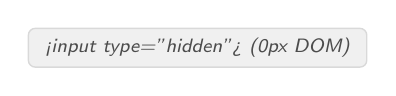
\begin{tikzpicture}[baseline=-0.5ex]
    \node[fill=gray!12, draw=gray!30, line width=0.5pt, rounded corners=2.5pt, inner xsep=6pt, inner ysep=3.5pt] 
      {\sffamily\scriptsize\textcolor{gray!60!black}{\textit{<input type="hidden"> (0px DOM)}}};
  \end{tikzpicture}%
}

\newcommand{\uiInputSubmit}{%
  \begin{tikzpicture}[baseline=-0.5ex]
    \fill[primaryBlue, rounded corners=3.5pt] (0, 0.05) rectangle (2.3, 0.55);
    \node[anchor=west, inner sep=0] at (0.22, 0.30) {\sffamily\bfseries\small\textcolor{white}{Gửi Dữ Liệu}};
    \fill[white] (1.92, 0.23) -- (1.92, 0.37) -- (2.04, 0.30) -- cycle;
  \end{tikzpicture}%
}

\newcommand{\uiInputReset}{%
  \begin{tikzpicture}[baseline=-0.5ex]
    \fill[white, draw=gray!40, line width=0.7pt, rounded corners=3.5pt] (0, 0.05) rectangle (1.9, 0.55);
    \draw[gray!70, line width=0.8pt] (0.35, 0.30) arc (160:-160:3.5pt);
    \fill[gray!70] (0.32, 0.38) -- (0.42, 0.38) -- (0.35, 0.46) -- cycle;
    \node[anchor=west, inner sep=0] at (0.58, 0.30) {\sffamily\bfseries\small\textcolor{gray!80!black}{Làm Lại}};
  \end{tikzpicture}%
}

\newcommand{\uiInputButton}{%
  \begin{tikzpicture}[baseline=-0.5ex]
    \fill[primaryBlue!6, draw=primaryBlue!50, line width=0.7pt, rounded corners=3.5pt] (0, 0.05) rectangle (2.0, 0.55);
    \node[anchor=center, inner sep=0] at (1.0, 0.30) {\sffamily\bfseries\small\textcolor{primaryBlue}{Click Action}};
  \end{tikzpicture}%
}

\newcommand{\uiInputImage}{%
  \begin{tikzpicture}[baseline=-0.5ex]
    \fill[accentOrange!10, draw=accentOrange!70, line width=0.7pt, rounded corners=3.5pt] (0, 0.05) rectangle (2.4, 0.55);
    \node[anchor=center, inner sep=0] at (1.2, 0.30) {\sffamily\bfseries\scriptsize\textcolor{accentOrange}{[IMG: Submit Button]}};
  \end{tikzpicture}%
}

